\subsection{El juego de la vida}

Para este experimento, se utiliza principalmente la regla B3/S23, de la cual fueron evolucionadas 100 condiciones iniciales aleatorias en un espacio de $100 \times 100$ durante 100 pasos evolutivos para analizar su comportamiento.  

De acuerdo con la figura \ref{fig:life_state_distribution}, la regla B3/S23 produce el estado uno un $16.5\%$ de las veces. La mayoría de los datos se agrupa entre $12.3\%$ y $20.7\%$, donde los porcentajes más grandes corresponden a las configuraciones iniciales aleatorias. Esto se demuestra en la figura \ref{fig:life_all_steps} donde la proporción del estado uno de todas las evoluciones a través del tiempo decrece hasta estabilizarse, comportamiento característico del atractor de dicha regla.

\begin{figure}[htbp]
	\centering
	\begin{subfigure}[b]{0.49\textwidth}
		\centering
		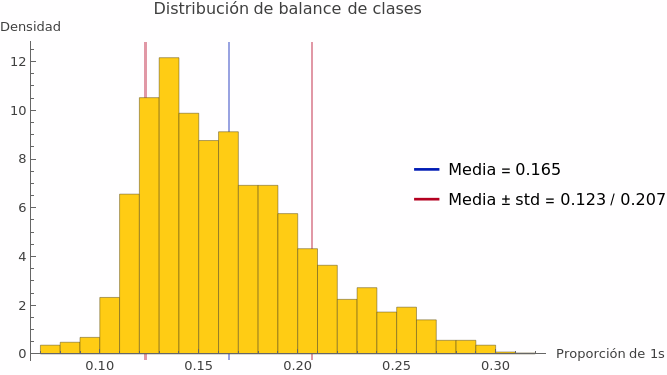
\includegraphics[width=\linewidth]{img/life_state_distribution.png}
		\caption{Histograma de distribución de la clase 1. Media de $16.5$ y desviación estándar de $4.2$.}
		\label{fig:life_state_distribution} 
	\end{subfigure}%
	\hfill % Añade espacio horizontal flexible entre las figuras
	\begin{subfigure}[b]{0.49\textwidth}
		\centering
		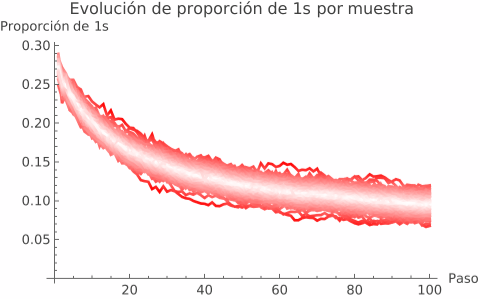
\includegraphics[width=\linewidth]{img/life_all_steps.png}
		\caption{Proporción de unos a lo largo del tiempo de todas las muestras.}
		\label{fig:life_all_steps}
	\end{subfigure}
	\caption{Resultados estadísticos del conjunto de pruebas para la regla B3/S23.}
\end{figure}

Por otro lado, dado que la salida de cada paso evolutivo es la entrada del siguiente, también se analiza el desbalance de entradas, es decir, la frecuencia con la que aparecen diferentes patrones. Para esto, utilizaremos la nomenclatura $CxNy$ que cuenta el número de unos que aparecen en el centro ($C$) y en el exterior ($N$).

En la figura \ref{fig:life_pattern_count} se muestran las frecuencias de aparición de todos los patrones en el mismo conjunto de datos. La regla B3/S23 no genera mucha vida dentro de las comunidades, lo que causa un desbalance de entradas. Los patrones con menor frecuencia de aparición son $C1N8$ y $C0N8$ sumando menos del $0.02\%$, lo que causa un problema de representación o sesgo de muestra.

\begin{figure}[H]
	\centering
	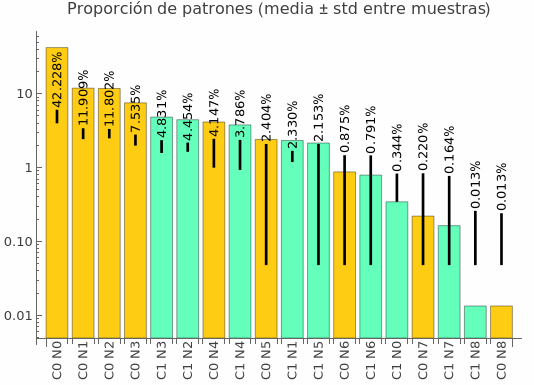
\includegraphics[width=0.7\linewidth]{img/life_pattern_count.png}
	\caption{Distribuciones de probabilidad de los patrones en la regla B3/S23.}
	\label{fig:life_pattern_count}
\end{figure}

Para evitar este sesgo, se proponen dos soluciones: (1) realizar un sobremuestreo de los datos menos frecuentes o (2) modificar la función de costo para penalizar en mayor medida los errores en patrones poco representados. Las pruebas a continuación se realizan con una pérdida objetivo exigente con la intención de encontrar configuraciones capaces de replicar el comportamiento de forma exacta.

\subsubsection{Capacidad de replicación}

Se usa la siguiente nomenclatura:
\[
\text{número de capas}:\text{número de neuronas}:\text{función de activación}
\]
para especificar la composición de la red neuronal. 

Fueron probadas 10 combinaciones de funciones de activación, de las cuales una sola converge en menos de 1,000 épocas. 
En la tabla \ref{tab:nca_gol_funciones_1} se observan los resultados. La falta de convergencia puede deberse al tamaño de la red neuronal o la pérdida objetivo utilizada. 

\begin{table}[h]
	\centering
	\begin{tabular}{llrrr}
		\toprule
		\textbf{Capa Oculta} & \textbf{Capa Salida} & \textbf{Épocas} & \textbf{Pérdida} & \textbf{Tiempo} \\
		\midrule
		1:4:ReLU & 2:Linear & 122 & 0.000098 & 4.64 s \\
		1:4:TanH & 1:Sigmoid & 1,000 & 0.052895 & 40.19 s\\
		1:4:TanH & 2:Linear & 1,000 & 0.079425 & 36.52 s \\
		1:4:Sigmoid & 2:Linear & 1,000 & 0.159343 & 36.71 s \\
		1:4:Sigmoid & 1:Sigmoid & 1,000 & 0.159343 & 39.37 s \\
		1:4:ReLU & 2:TanH & 1,000 &  0.179589 & 38.65 s \\
		1:4:ReLU & 1:Sigmoid & 1,000 & 0.269196 & 38.16 s\\
		1:4:Linear & 1:Sigmoid & 1,000 & 0.297529 & 39.12 s \\
		1:4:Linear & 2:Linear & 1,000 & 0.297529 & 34.75 s  \\
		1:4:ReLU & 2:Sigmoid & 1,000 & 0.374756 & 37.55 s \\
		\bottomrule
	\end{tabular}
	\caption{Comparativa de rendimiento con múltiples hiperparámetros de la regla B3/S23: pérdida objetivo 0.0001, límite de épocas: 1,000,
		tamaño del lote: 8,192, tasa de aprendizaje: 0.001, semilla aleatoria: 42.}
	\label{tab:nca_gol_funciones_1}
\end{table}

Al incrementar el número de capas ocultas y de neuronas, se observa en la tabla \ref{tab:nca_gol_funciones_2} que existen cuatro nuevas configuraciones que alcanzan la convergencia. Adicionalmente, en la figura \ref{fig:gol_funciones_2} observamos que el estancamiento ocurre en las primeras 12 épocas, lo que sugiere un problema de la combinación de funciones de activación más que una limitación de la tasa de aprendizaje. 

\begin{table}[h]
	\centering
	\begin{tabular}{llrr}
		\toprule
		\textbf{Capa Oculta} & \textbf{Capa Salida} & \textbf{Épocas} & \textbf{Pérdida}\\
		\midrule
		4:8:ReLU & 2:Linear & 18 & 0.000087 \\
		4:8:TanH & 1:Sigmoid & 51 & 0.000097 \\
		4:8:TanH & 2:Linear & 35 & 0.000097 \\
		4:8:Sigmoid & 2:Linear & 79 & 0.000095 \\
		4:8:Sigmoid & 1:Sigmoid & 1,000 & 0.159342 \\
		4:8:ReLU & 2:TanH & 1,000 & 0.126928 \\
		4:8:ReLU & 1:Sigmoid & 133 & 0.000096 \\
		4:8:Linear & 1:Sigmoid & 1,000 & 0.297542 \\
		4:8:Linear & 2:Linear & 1,000 & 0.297544 \\
		4:8:ReLU & 2:Sigmoid & 1,000 & 0.374756 \\
		\bottomrule
	\end{tabular}
	\caption{Comparativa de rendimiento con múltiples hiperparámetros de la regla B3/S23: pérdida objetivo 0.0001, límite de épocas: 1,000,
		tamaño del lote: 8,192, tasa de aprendizaje: 0.001, semilla aleatoria: 42.}
	\label{tab:nca_gol_funciones_2}
\end{table}

\begin{figure}[H]
	\centering
	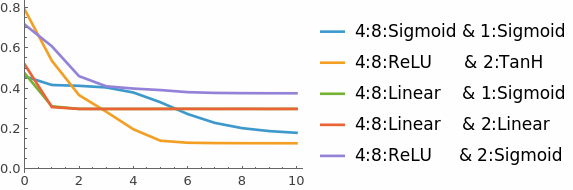
\includegraphics[width=0.75\linewidth]{img/gol_funciones_2.png}
	\caption{Registro de pérdida obtenida en las primeras 12 épocas de las configuraciones sin convergencia de la tabla \ref{tab:nca_gol_funciones_2}.}
	\label{fig:gol_funciones_2}
\end{figure}

Queda demostrado que un autómata celular neuronal puede aprender el comportamiento de una regla ya conocida con una pérdida de 0.0001. Para fines de esta investigación, se omiten las configuraciones no convergentes.

\subsubsection{Aprendizaje de reglas similares}

De acuerdo con la figura \ref{fig:life_pattern_count}, las probabilidades de aparición de los patrones $C0N8$ y $C1N8$ son menores que $0.02\%$. La siguiente prueba busca identificar la relación entre la pérdida objetivo y la regla aprendida. Para esto, se entrena la regla B3/S23 con diferentes pérdidas objetivo y se identifica cómo esos patrones infrecuentes afectan el aprendizaje.

Cabe mencionar que aunque las reglas del juego de la vida son semitotalísticas, existe la posibilidad de que la regla aprendida no lo sea, es decir, el autómata celular neuronal sí haga distinción entre dos patrones que conduzcan al mismo comportamiento. Por ejemplo, podemos generar de ocho formas diferentes el patrón $C0N1$:
\[
 \left[ \begin{matrix} 1 & 0 & 0 \\ 0 & 0 & 0 \\ 0 & 0 & 0 \end{matrix} \right] = 
 \left[ \begin{matrix} 0 & 1 & 0 \\ 0 & 0 & 0 \\ 0 & 0 & 0 \end{matrix} \right] = \dots = 
 \left[ \begin{matrix} 0 & 0 & 0 \\ 0 & 0 & 0 \\ 0 & 0 & 1 \end{matrix} \right]
\]
 pero a falta de exposición de todas las posibles configuraciones, la red neuronal puede distinguir patrones, convirtiendo a la regla en una arbitraria.
 
Las reglas semitotalísticas son un subconjunto de las reglas arbitrarias. Para verificar que la regla aprendida coincida con todas las posibles configuraciones de los patrones, se diseñó la configuración inicial de la figura \ref{fig:test}, la cual se evoluciona un paso y se comparan los centros de cada subespacio de $3 \times 3$. 

\begin{figure}[H]
	\centering
	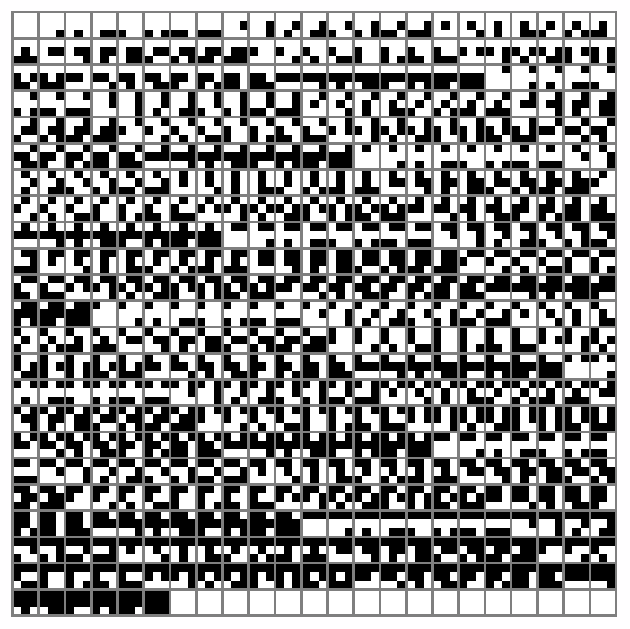
\includegraphics[width=0.6\linewidth]{img/test.png}
	\caption{Espacio que contiene todas las configuraciones posibles ($2^9 = 512$) de 2 estados en 9 células.}
	\label{fig:test}
\end{figure}

Los autómatas celulares neuronales que utilizaron la pérdida objetivo de 0.2 y 0.3 aprendieron la regla 0 (ver figura \ref{fig:b3s23_loss}). Podemos concluir que esta configuración es estable porque, aunque existan patrones de baja frecuencia como $C0N8$ y $C1N8$, sigue siendo capaz de replicar el comportamiento con una pérdida objetivo de $0.1$. Una hipótesis es que la red neuronal se inicializa generando ceros y, como casi nunca recibe esas entradas, sus salidas para ellas se mantienen en ese valor. 

\begin{figure}[H]
	\centering
	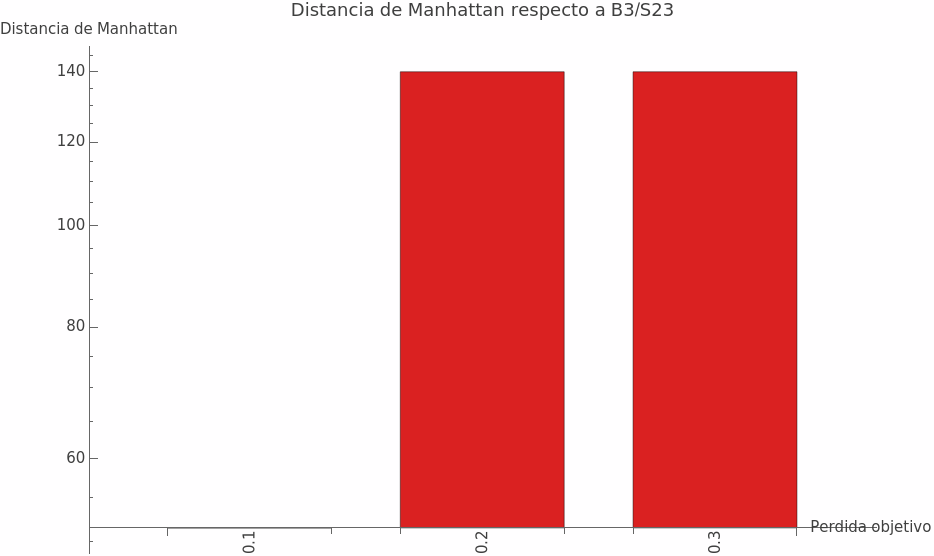
\includegraphics[width=0.6\linewidth]{img/b3s23_loss.png}
	\caption{Distancia Manhattan de los vectores de regla de múltiples pérdidas objetivo comparados con B3/S23.}
	\label{fig:b3s23_loss}
\end{figure}


A continuación, se replica el experimento para las siguientes reglas \textit{life-like}: B3/S238, B38/S238 y B3/S236.

La regla B3/S238 (figura \ref{fig:b3s238_loss}) aprende una regla que difiere únicamente en un elemento (con una pérdida objetivo entre 0.03 y 0.1). Esta diferencia corresponde al patrón $C1N8$, el cual solo tiene una posible representación:
\[
\left[
\begin{matrix}
	1 & 1 & 1 \\
	1 & 1 & 1 \\
	1 & 1 & 1 
\end{matrix}
\right]
\]

\begin{figure}[H]
	\centering
	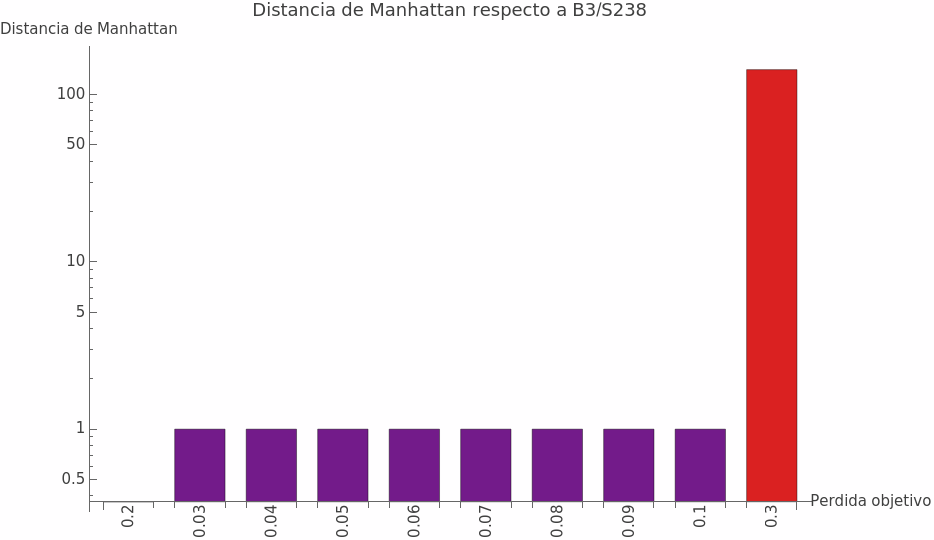
\includegraphics[width=.6\linewidth]{img/b3s238_loss.png}
	\caption{Distancia Manhattan de los vectores de regla de múltiples pérdidas objetivo comparados con B3/S238.}
	\label{fig:b3s238_loss} 
\end{figure}

Como la regla aprendida considera todas las permutaciones del patrón $C1N8$, significa que aprendió una regla semitotalística que ignora supervivencia con 8 vecinos. Su regla aprendida equivale a B3/S23. Esto lo corroboramos con la figura \ref{fig:b3s238_vector}, en donde se muestra la única diferencia entre ambas reglas y cómo fue omitida durante el entrenamiento. 

\begin{figure}[H]
	\centering
	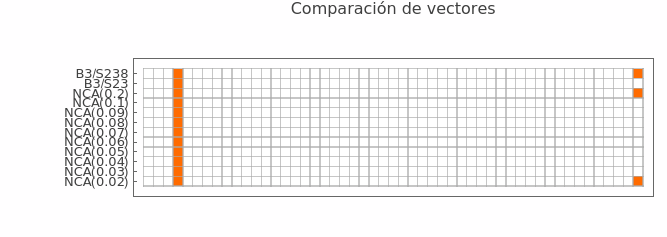
\includegraphics[width=.8\linewidth]{img/b3s238_vector.png}
	\caption{Últimos 50 elementos de los vectores de regla de B3/S238, B3/S23 y los aprendidos por el autómata celular neuronal.}
	\label{fig:b3s238_vector} 
\end{figure}

La regla B38/S238 (figura \ref{fig:b38s238_loss}) aprende 2 comportamientos diferentes: B3/S238 y B3/S23, como se observa en la figura \ref{fig:b38s238_vector}.

\begin{figure}[H]
	\centering
	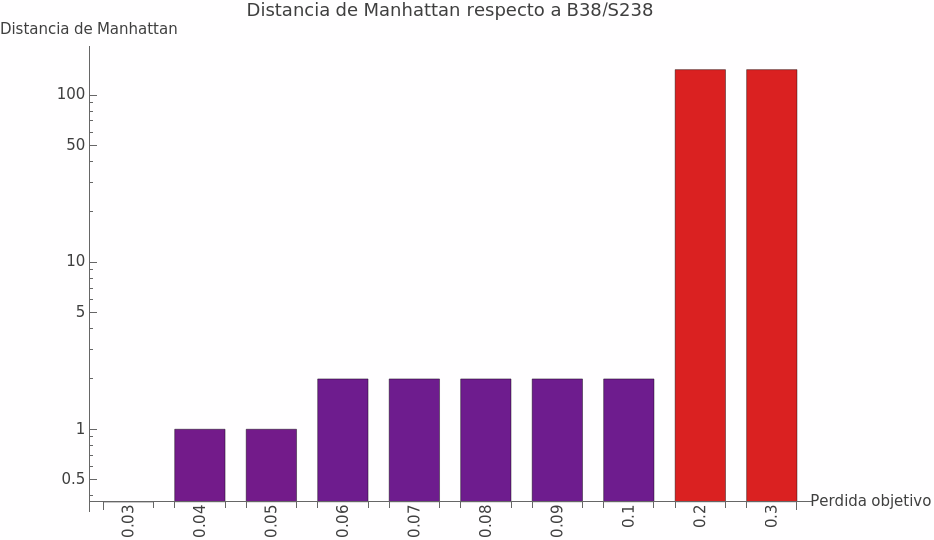
\includegraphics[width=.6\linewidth]{img/b38s238_loss.png}
	\caption{Distancia Manhattan de los vectores de regla de múltiples pérdidas objetivo comparados con B38/S238.}
	\label{fig:b38s238_loss} 
\end{figure}

\begin{figure}[H]
	\centering
	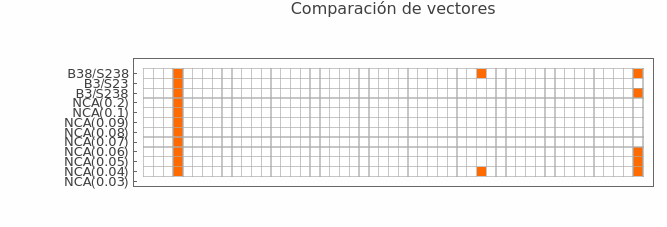
\includegraphics[width=.8\linewidth]{img/b38s238_vector.png}
	\caption{Últimos 50 elementos de los vectores de regla de B38/S238, B3/S23, B3/S238 y los aprendidos por el autómata celular neuronal.}
	\label{fig:b38s238_vector} 
\end{figure}

En la regla B3/S236 (figura \ref{fig:b3s236_loss}) con 0.2 difieren 32 elementos, de los cuales 28 sustituyeron el 1 por 0 (figura \ref{fig:b3s236_02_10}) y 4 al revés (figura \ref{fig:b3s236_02_01}). El primer conjunto corresponde al patrón $C1N6$, mientras que los 4 restantes necesitan otros 4 patrones adicionales para capturar a $C1N7$. Por esta razón, la regla aprendida no es semitotalística, porque hace distinción entre elementos de su vecindad.

\begin{figure}[H]
	\centering
	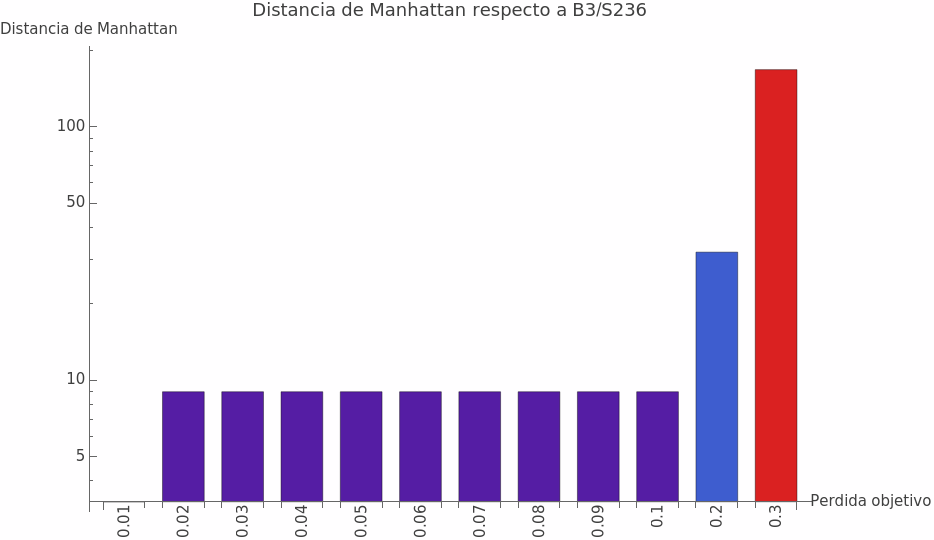
\includegraphics[width=.75\linewidth]{img/b3s236_loss.png}
	\caption{Distancia Manhattan de los vectores de regla de múltiples pérdidas objetivo comparados con B3/S236.}
	\label{fig:b3s236_loss} 
\end{figure}

\begin{figure}[htbp]
	\centering
	\begin{subfigure}[b]{0.5\textwidth}
		\centering
		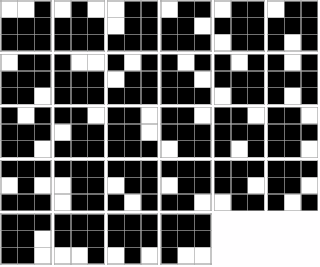
\includegraphics[width=0.7\linewidth]{img/b3s236_02_10.png}
		\caption{Se intercambió 1 por 0 en $C1N6$.}
		\label{fig:b3s236_02_10} 
	\end{subfigure}%
	\hfill % Añade espacio horizontal flexible entre las figuras
	\begin{subfigure}[b]{0.5\textwidth}
		\centering
		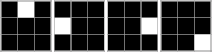
\includegraphics[width=0.5\linewidth]{img/b3s236_02_01.png}
		\caption{Se intercambió 0 por 1.}
		\label{fig:b3s236_02_01}
	\end{subfigure}
	\caption{Patrones que difieren entre B3/S236 y el autómata celular neuronal con una pérdida objetivo de 0.2.}
\end{figure}

El resto de reglas aprendidas erróneamente (con pérdidas objetivo de 0.02 a 0.1) diferencian los patrones de las figuras \ref{fig:b3s236_03_10} y \ref{fig:b3s236_03_01}. Ambos patrones se encuentran completos ($C1N7$ y $C1N8$), por lo que sobrevive con 7 y 8 vecinos, es decir, aprendió la regla B3/S23678.

\begin{figure}[htbp]
	\centering
	\begin{subfigure}[b]{0.5\textwidth}
		\centering
		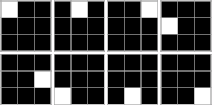
\includegraphics[width=0.7\linewidth]{img/b3s236_03_10.png}
		\caption{Se intercambió 0 por 1 en $C1N7$.}
		\label{fig:b3s236_03_10} 
	\end{subfigure}%
	\hfill % Añade espacio horizontal flexible entre las figuras
	\begin{subfigure}[b]{0.5\textwidth}
		\centering
		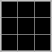
\includegraphics[width=0.17\linewidth]{img/b3s236_03_01.png}
		\caption{Se intercambió 0 por 1 en $C1N8$.}
		\label{fig:b3s236_03_01}
	\end{subfigure}
	\caption{Patrones que difieren entre B3/S236 y el autómata celular neuronal con pérdidas objetivo de 0.02 a 0.1.}
\end{figure}

\subsubsection{Efecto del tamaño de la vecindad}

Experimentar con reglas ya conocidas implica conocer toda la configuración necesaria de ese sistema en específico. Esto no ocurre en fenómenos reales donde no conocemos el número de estados, la función de transición o, específicamente para este experimento, la vecindad que define el sistema. Los siguientes experimentos tienen el propósito de identificar cómo afecta el desconocimiento de la vecindad en un sistema complejo al momento de intentar replicar el comportamiento de la regla B3/S23.

Dada la vecindad de la regla, definimos las siguientes pruebas: (1) eliminación de una célula exterior, (2) eliminación de la célula central, (3) incremento del tamaño de la vecindad y (4) sustitución de elementos de la vecindad. Con esto se busca identificar un método de selección de vecindad que nos permita extraer el comportamiento esencial de un sistema complejo.

La vecindad semitotalística se divide en dos subvecindades, el centro y los bordes. Dado que el valor de la subvecindad de los bordes está dado por la sumatoria, cada uno de ellos tiene la misma relevancia, por lo que solo es necesario realizar pruebas ignorando uno de esos elementos. La tabla \ref{tab:vecindad_ajuste_16x16} muestra las pérdidas finales obtenidas bajo diferentes configuraciones, todas mayores a 0.1. 

\begin{table}[H]
	\centering
	\small
	\begin{tabular}{ccccccc}
		\toprule
		& & \textbf{ReLU} & \textbf{TanH} & \textbf{TanH} & \textbf{ReLU} &  \\
		\textbf{Tasa} & \textbf{Lote} & \textbf{2:Linear }&  \textbf{1:Sigmoid }& \textbf{2:Linear  }& \textbf{1:Sigmoid} & \textbf{Segundos}  \\
		\midrule
		0.0003 & 1,024 & 0.121595 & 0.121808 & 0.121824 & 0.121536 & 216 \\
		0.0003 & 4,096 & 0.121675 & 0.122049 & 0.122123 & 0.121576 & 58 \\
		0.0003 & 8,192 & 0.121774 & 0.122444 & 0.122367 & 0.121747 & 40 \\
		\midrule
		0.001 & 1,024 & 0.121590 & 0.121645 & 0.121871 & 0.121605 & 213 \\
		0.001 & 4,096 & 0.121546 & 0.121790 & 0.121768 & 0.121580 & 58 \\
		0.001 & 8,192 & 0.121794 & 0.121946 & 0.122043 & 0.121604 & 42 \\
		\midrule
		0.003 & 1,024 & 0.121685 & 0.414336 & 0.414441 & 0.486924 & 210 \\
		0.003 & 4,096 & 0.121647 & 0.230796 & 0.318269 & 0.121626 & 58 \\
		0.003 & 8,192 & 0.192933 & 0.122014 & 0.122387 & 0.121660 & 35 \\
		\bottomrule
	\end{tabular}
	\caption{Pérdida final de cada configuración. Vecindad de $3 \times 3$ sin el vecino noroeste, 100 épocas, semilla 42, red de tamaño 16:16. Pérdida mínima alcanzable: 0.121294.}
	\label{tab:vecindad_ajuste_16x16}
\end{table}

Como se mencionó anteriormente, con una pérdida objetivo de 0.1 la red neuronal aún replica B3/S23; en este caso ninguna configuración baja de 0.12, por lo que la red neuronal no pudo replicar el comportamiento. Todas las configuraciones del barrido sin el vecino noroeste (de 1:4 a 16:16, con las cuatro combinaciones de funciones de activación) aprenden la misma regla, que difiere en 98 de 512 elementos ($19\%$). La regla aprendida no genera osciladores, sino únicamente produce naturaleza muerta. 

Si ignoramos la célula central (tabla \ref{tab:vecindad_centro}) observamos que ninguna de las configuraciones tuvo una pérdida menor a 0.07, mucho menor que eliminando un vecino del exterior. Es una bella casualidad cómo mediante este experimento, se demuestra una vez más que existe una mayor dependencia de los estados vecinos que del propio. La regla aprendida tiende a eliminar todos los estados 1 y genera pocas configuraciones estáticas y cíclicas en menos de 50 pasos, tal como se muestra en la figura \ref{fig:b3s23_c0n8}.

\begin{table}[H]
	\centering
	\begin{tabular}{llr}
		\toprule
		\textbf{Capa Oculta} & \textbf{Capa Salida} & \textbf{Pérdida} \\ 
			\midrule
			1:4:ReLU & 2:Linear & 0.088437 \\
			2:8:ReLU & 2:Linear & 0.085921 \\
			4:8:ReLU & 2:Linear & 0.078934 \\
			4:16:ReLU & 2:Linear & 0.078685 \\
			8:16:ReLU & 2:Linear & 0.078674 \\
			16:16:ReLU & 2:Linear & 0.078720 \\
			\midrule
			1:4:TanH & 1:Sigmoid & 0.081676 \\
			2:8:TanH & 1:Sigmoid & 0.078866 \\
			4:8:TanH & 1:Sigmoid & 0.078713 \\
			4:16:TanH & 1:Sigmoid & 0.078670 \\
			8:16:TanH & 1:Sigmoid & 0.078671 \\
			16:16:TanH & 1:Sigmoid & 0.078707 \\
			\midrule
			1:4:TanH & 2:Linear & 0.082283 \\
			2:8:TanH & 2:Linear & 0.078758 \\
			4:8:TanH & 2:Linear & 0.078716 \\
			4:16:TanH & 2:Linear & 0.078685 \\
			8:16:TanH & 2:Linear & 0.078680 \\
			16:16:TanH & 2:Linear & 0.078900 \\
			\midrule
			1:4:ReLU & 1:Sigmoid & 0.168493 \\
			2:8:ReLU & 1:Sigmoid & 0.080522 \\
			4:8:ReLU & 1:Sigmoid & 0.078796 \\
			4:16:ReLU & 1:Sigmoid & 0.078688 \\
			8:16:ReLU & 1:Sigmoid & 0.078679 \\
			16:16:ReLU & 1:Sigmoid & 0.078671 \\
			\bottomrule
		\end{tabular}
		\caption{Regla B3/S23 sin la célula central. Pérdida objetivo 0.001, límite de épocas: 500, tamaño del lote: 4,096, tasa de aprendizaje: 0.001, semilla aleatoria: 42. Pérdida mínima alcanzable: 0.078650.}
		\label{tab:vecindad_centro}
	\end{table}

\begin{figure}[htbp]
	\centering
	\begin{subfigure}[b]{0.5\textwidth}
		\centering
		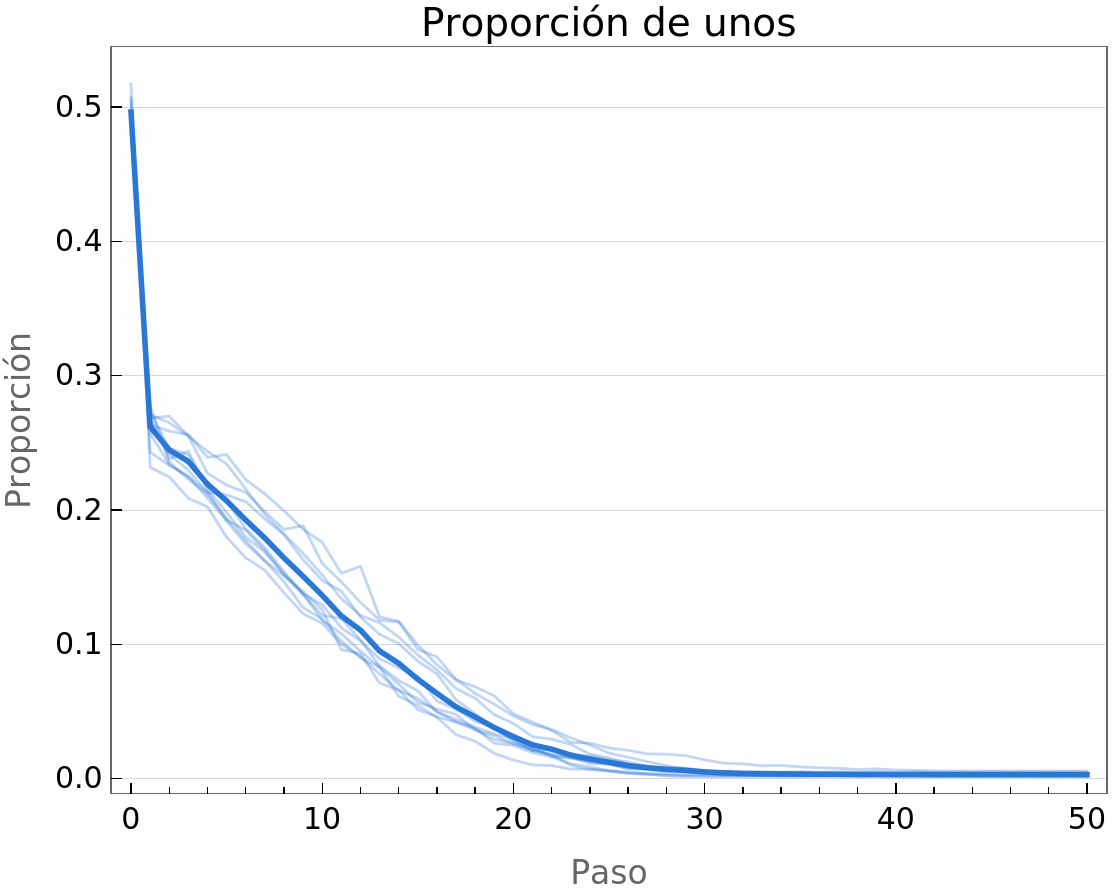
\includegraphics[width=0.77\linewidth]{img/b3s23_reduction_1s.png}
		\caption{Proporción de unos en cada paso evolutivo.}
		\label{fig:b3s23_reduction_1s} 
	\end{subfigure}%
	\hfill % Añade espacio horizontal flexible entre las figuras
	\begin{subfigure}[b]{0.5\textwidth}
		\centering
		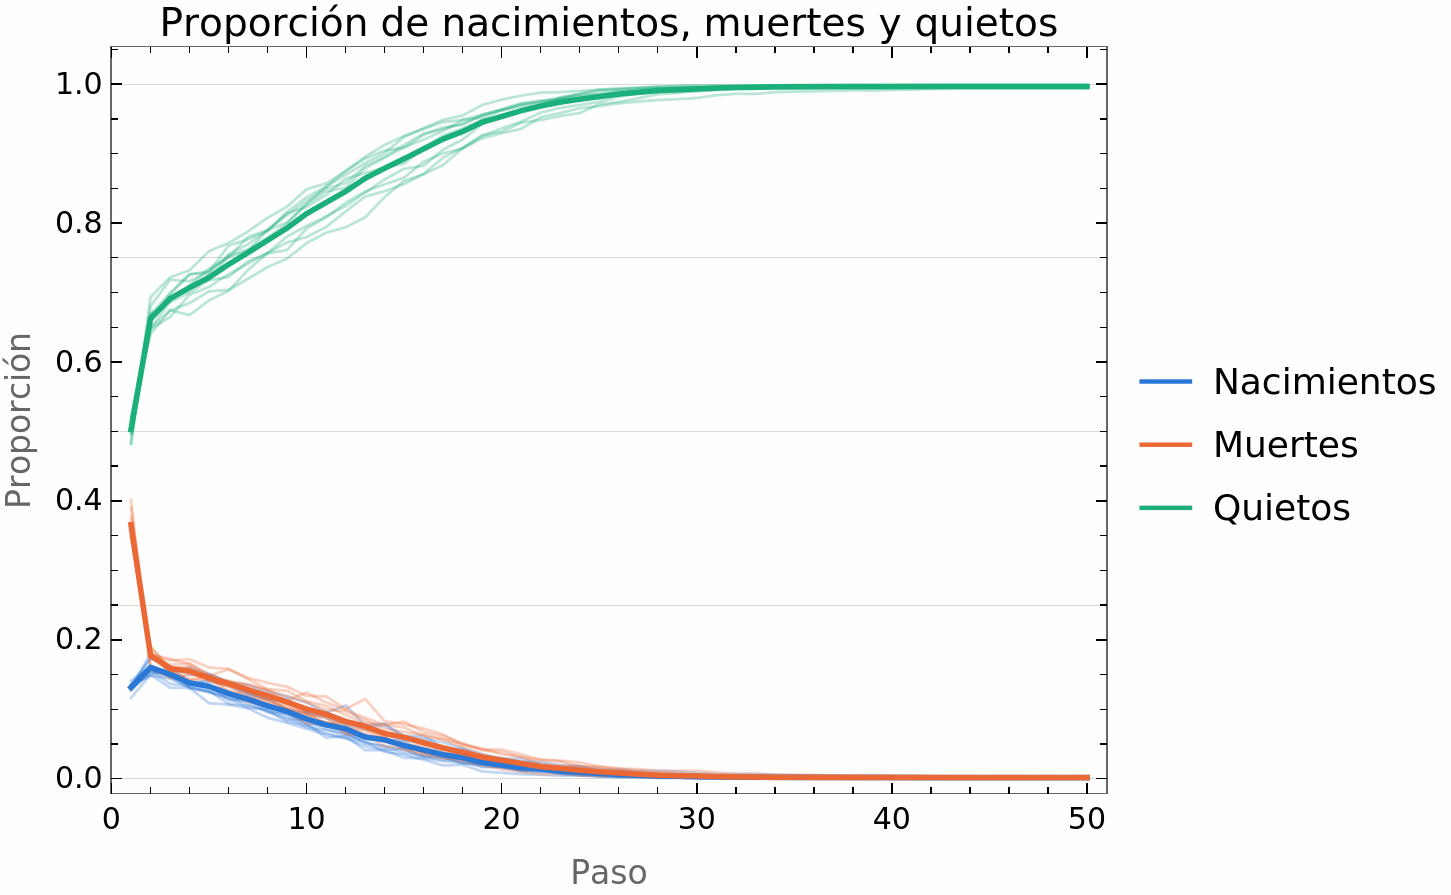
\includegraphics[width=\linewidth]{img/b3s23_reduction_changes.png}
		\caption{Porcentaje de nacimientos, muertes y células sin cambios en cada paso evolutivo.}
		\label{fig:b3s23_reduction_changes}
	\end{subfigure}
	\caption{Proporciones de estados y cambios de estados en 10 evoluciones con condiciones iniciales aleatorias durante 50 pasos con el autómata celular neuronal obtenido por 16:16:ReLU \& 1:Sigmoid.}
	\label{fig:b3s23_c0n8}
\end{figure}

Por otro lado, el incremento de la vecindad no afecta la replicación del comportamiento. La red neuronal puede aprender la regla incluso con exceso de información. En la tabla \ref{tab:vecindad_ampliada} se muestran los mejores resultados con sus respectivas pérdidas finales, todas alcanzaron la pérdida objetivo en 21 épocas o menos.

\begin{table}[H]
	\centering
	\footnotesize
	\begin{tabular}{lllr}
		\toprule
		\textbf{Vecindad} & \textbf{Capa Oculta} & \textbf{Capa Salida} & \textbf{Pérdida} \\
		\midrule
		\multirow{3}{*}{$5\times5$} & 4:16:ReLU & 2:Linear & 0.000035 \\
		& 8:16:ReLU & 2:Linear & 0.000062 \\
		& 16:16:ReLU & 1:Sigmoid & 0.000225 \\
		\midrule
		\multirow{3}{*}{$7\times7$} & 8:16:ReLU & 2:Linear & 0.000023 \\
		& 8:16:ReLU & 1:Sigmoid & 0.000045 \\
		& 4:16:ReLU & 1:Sigmoid & 0.000137 \\
		\midrule
		\multirow{3}{*}{$8\times8$} & 8:16:ReLU & 2:Linear & 0.000063 \\
		& 8:16:ReLU & 1:Sigmoid & 0.000141 \\
		& 16:16:ReLU & 1:Sigmoid & 0.000156 \\
		\bottomrule
	\end{tabular}
	\caption{Las tres configuraciones con menor pérdida de la regla B3/S23 al aumentar la vecindad. Pérdida objetivo 0.001, límite de épocas: 500, tamaño del lote: 4,096, tasa de aprendizaje: 0.001, semilla aleatoria: 42. La vecindad de $8\times8$ abarca los desplazamientos $-4$ a $3$ en cada eje.}
	\label{tab:vecindad_ampliada}
\end{table}

Para finalizar, se realiza la sustitución, es decir, se elimina un elemento de la vecindad, pero se compensa con un incremento de vecinos circundantes en ese punto faltante. Esto con el objetivo de analizar si la información adicional es útil o es únicamente ruido.

En la tabla \ref{tab:vecindad_reducida_ampliada} se experimenta con vecindades de $7 \times 7$ y $9 \times 9$ ignorando en cada caso un vecino: la esquina noroeste $(-1,-1)$ o el centro $(0,0)$. Se aprecia que el incremento de la vecindad reduce parcialmente la pérdida. Para el centro, pasamos de un 0.078650 a un 0.065987, y para el borde de 0.121294 a 0.097587.

\begin{table}[H]
	\centering
	\footnotesize
	\begin{tabular}{lllr}
		\toprule
		\textbf{Vecindad} & \textbf{Capa Oculta} & \textbf{Capa Salida} & \textbf{Pérdida} \\
		\midrule
		\multirow{4}{*}{$7\times7$ sin $(-1,-1)$} & 16:16:ReLU & 2:Linear & 0.099847 \\
		& 16:16:TanH & 1:Sigmoid & 0.098628 \\
		& 16:16:TanH & 2:Linear & 0.098407 \\
		& 16:16:ReLU & 1:Sigmoid & 0.099326 \\
		\midrule
		\multirow{4}{*}{$9\times9$ sin $(-1,-1)$} & 16:16:ReLU & 2:Linear & 0.098381 \\
		& 16:16:TanH & 1:Sigmoid & 0.097587 \\
		& 16:16:TanH & 2:Linear & 0.098029 \\
		& 16:16:ReLU & 1:Sigmoid & 0.098368 \\
		\midrule
		\multirow{4}{*}{$7\times7$ sin $(0,0)$} & 16:16:ReLU & 2:Linear & 0.067663 \\
		& 16:16:TanH & 1:Sigmoid & 0.066962 \\
		& 16:16:TanH & 2:Linear & 0.066976 \\
		& 16:16:ReLU & 1:Sigmoid & 0.068002 \\
		\midrule
		\multirow{4}{*}{$9\times9$ sin $(0,0)$} & 16:16:ReLU & 2:Linear & 0.067066 \\
		& 16:16:TanH & 1:Sigmoid & 0.066031 \\
		& 16:16:TanH & 2:Linear & 0.065987 \\
		& 16:16:ReLU & 1:Sigmoid & 0.067197 \\
		\bottomrule
	\end{tabular}
	\caption{Regla B3/S23 con vecindades de $7\times7$ y $9\times9$ sin un vecino. Pérdida objetivo 0.001, límite de épocas: 500, tamaño del lote: 4,096, tasa de aprendizaje: 0.001, semilla aleatoria: 42.}
	\label{tab:vecindad_reducida_ampliada}
\end{table}

Con estos resultados experimentales, establecemos algunas consideraciones esenciales para el entrenamiento de autómatas celulares neuronales:

\begin{itemize}
	\item La capacidad de generalización depende de clases y entradas balanceadas. Establecer una pérdida objetivo restrictiva fuerza a la red a ajustar sus pesos en regiones con patrones menos representados. El caso contrario atenúa estados y los conduce a otros comportamientos. 
	
	\item El entrenamiento de reglas semitotalísticas no garantiza que la regla aprendida igual lo sea. 

	\item Incrementar el tamaño de la vecindad es un costo computacional viable cuando se desconoce el tamaño de la vecindad real. El incremento de igual manera puede ayudar a disminuir la pérdida si es que aún existen vecinos que no fueron considerados pero con un límite contextual.

\end{itemize}

Estos experimentos confirman que no se requieren arquitecturas neuronales complejas para replicar este tipo de dinámicas evolutivas. Asimismo, queda validada la metodología propuesta para extraer e identificar el vector de regla aprendido por el modelo, sentando las bases para los siguientes experimentos del capítulo.
